\documentclass[../../../OAE-SPEC-MAIN.tex]{subfiles}
\begin{document}

\section{FPGA Implementation Specification (Conventional Ethernet)}

This appendix provides detailed specifications for implementing the CQ protocol in a Conventional Ethernet packet format in an FPGA, suitable for testing and evaluation.

\subsection{Frame Format (Conventional Ethernet)}


\begin{table}[h]
%\centering
\hspace{-8pt}
\begin{tabular}{|l|c|l|}
\hline
\textbf{Field} & \textbf{Size (bits)} & \textbf{Description} \\
\hline
Preamble* & 64 & Standard Ethernet preamble with SFD \\
Destination MAC* & 48 & Destination MAC address \\
Source MAC* & 48 & Source MAC address \\
EtherType* & 16 & Custom EtherType (0xCQ01) \\
Balance Indicator & 3 & Encoded balance state \\
Operation Code & 5 & Operation type \\
Transaction ID & 16 & Unique transaction identifier \\
Payload Length & 16 & Length of payload in bytes \\
Payload & Variable & Data payload (if applicable) \\
CRC & 32 & Frame check sequence \\
\hline
\end{tabular}
\caption{CQ Protocol Frame Format. \\  \vspace{5pt} *Not Needed in Æ-Link Interconnects. Source \& destination identifiers are redundant between adjacent Æ Cells. \\i.e. Software Endpoints Directly Connected over a single link where (\emph{private} identities and identifiers are in pre-frame negotiation).}
\end{table}


\subsection{Balance Indicator Encoding}

\begin{table}[h]
\centering
\begin{tabular}{|c|l|}
\hline
\textbf{Value} & \textbf{Meaning} \\
\hline
000 & $-\infty$ (Complete deficit) \\
001 & $-1$ (Specific deficit) \\
010 & $-0$ (Balance with negative tendency) \\
011 & $+0$ (Balance with positive tendency) \\
100 & $+1$ (Specific surplus) \\
101 & $+\infty$ (Complete surplus) \\
110-111 & Reserved \\
\hline
\end{tabular}
\caption{Balance Indicator Encoding}
\end{table}

\subsection{Operation Code Encoding}

\begin{table}[h]
\centering
\begin{tabular}{|c|l|}
\hline
\textbf{Value} & \textbf{Operation} \\
\hline
00000 & NOP (No Operation) \\
00001 & DATA (Data Transfer) \\
00010 & ACK (Acknowledgment) \\
00011 & REQ (Request for Data) \\
00100 & RSP (Response to Request) \\
00101 & SYNC (Synchronization) \\
00110 & SYNC\_ACK (Synchronization Acknowledgment) \\
00111 & RESET (Connection Reset) \\
01000-11111 & Reserved \\
\hline
\end{tabular}
\caption{Operation Code Encoding}
\end{table}

\subsection{State Machine Definition}

The core state machine for the CQ protocol implementation is defined as follows:

\begin{figure}[ht]
\centering
\begin{tikzpicture}[node distance=2cm, auto, 
                    every state/.style={draw=black!60, very thick, fill=white!20},
                    ->, >=stealth]
    \node[state] (INIT) {INIT};
    \node[state, right=3cm of INIT] (ZERO_POS) {$+0$};
    \node[state, above right=of ZERO_POS] (POS_ONE) {$+1$};
    \node[state, below right=of ZERO_POS] (NEG_ONE) {$-1$};
    \node[state, right=3cm of ZERO_POS] (ZERO_NEG) {$-0$};
    \node[state, above right=of ZERO_NEG] (POS_INF) {$+\infty$};
    \node[state, below right=of ZERO_NEG] (NEG_INF) {$-\infty$};

    \draw (INIT) -- node[above] {SYNC} (ZERO_POS);
    \draw (ZERO_POS) -- node[above left] {Send} (POS_ONE);
    \draw (POS_ONE) -- node[below right] {ACK} (ZERO_POS);
    \draw (ZERO_POS) -- node[below left] {Request} (NEG_ONE);
    \draw (NEG_ONE) -- node[above right] {Receive} (ZERO_POS);
    \draw (ZERO_POS) -- node[above] {SYNC\_ACK} (ZERO_NEG);
    \draw (ZERO_NEG) -- node[above left] {Receive} (POS_INF);
    \draw (POS_INF) -- node[below right] {Process} (ZERO_NEG);
    \draw (ZERO_NEG) -- node[below left] {Request} (NEG_INF);
    \draw (NEG_INF) -- node[above right] {Send} (ZERO_NEG);
    
    \draw (ZERO_POS) to[out=135, in=225, looseness=5] node[left] {Timeout} (ZERO_POS);
    \draw (ZERO_NEG) to[out=45, in=315, looseness=5] node[right] {Timeout} (ZERO_NEG);
\end{tikzpicture}
\caption{CQ Protocol State Machine}
\end{figure}

\subsection{FPGA Implementation Architecture}

\begin{figure}[h]
\centering
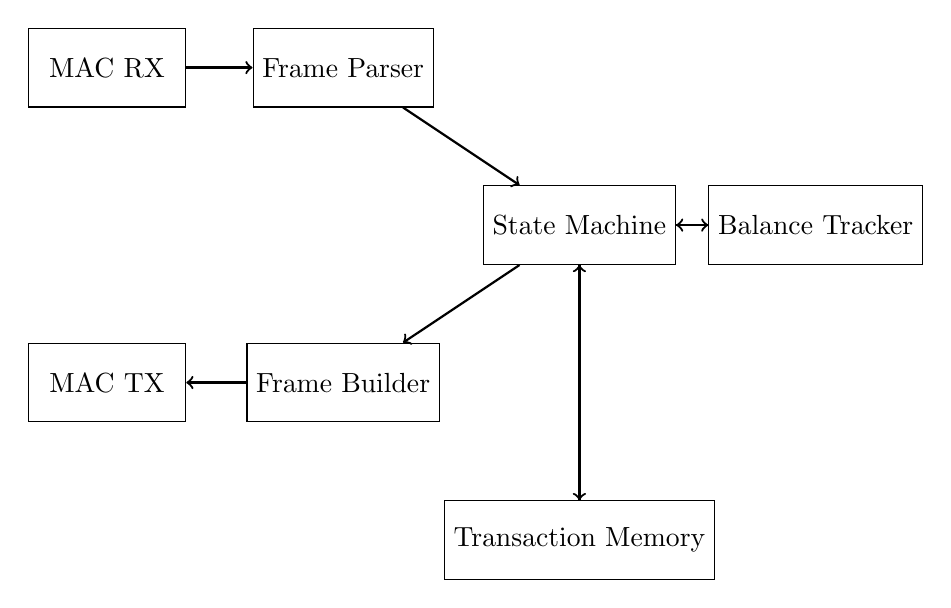
\begin{tikzpicture}[
    module/.style={rectangle, draw, text centered, minimum height=1cm, minimum width=2cm},
    arrow/.style={->, thick}
]
    % Input/Output modules
    \node[module] (mac_rx) at (0,0) {MAC RX};
    \node[module] (mac_tx) at (0,-4) {MAC TX};
    
    % Protocol modules
    \node[module] (frame_parser) at (3,0) {Frame Parser};
    \node[module] (frame_builder) at (3,-4) {Frame Builder};
    
    % Core logic
    \node[module] (state_machine) at (6,-2) {State Machine};
    \node[module] (balance_tracker) at (9,-2) {Balance Tracker};
    
    % Memory
    \node[module] (transaction_memory) at (6,-6) {Transaction Memory};
    
    % Connections
    \draw[arrow] (mac_rx) -- (frame_parser);
    \draw[arrow] (frame_parser) -- (state_machine);
    \draw[arrow] (state_machine) -- (balance_tracker);
    \draw[arrow] (balance_tracker) -- (state_machine);
    \draw[arrow] (state_machine) -- (frame_builder);
    \draw[arrow] (frame_builder) -- (mac_tx);
    \draw[arrow] (state_machine) -- (transaction_memory);
    \draw[arrow] (transaction_memory) -- (state_machine);
\end{tikzpicture}
\caption{FPGA Implementation Architecture}
\end{figure}

\subsection{Registers and Memory Structure}

\begin{table}[h]
\centering
\begin{tabular}{|l|c|l|}
\hline
\textbf{Register} & \textbf{Width (bits)} & \textbf{Description} \\
\hline
STATE\_REG & 3 & Current protocol state \\
BALANCE\_REG & 3 & Current balance indicator \\
TRANS\_ID\_REG & 16 & Current transaction ID \\
TIMEOUT\_COUNTER & 32 & Timeout counter \\
CONTROL\_REG & 8 & Control register \\
STATUS\_REG & 8 & Status register \\
\hline
\end{tabular}
\caption{Register Definitions}
\end{table}

\subsection{Memory Organization}

The Transaction Memory should be implemented as dual-port RAM with the following structure:

\begin{table}[h]
\centering
\begin{tabular}{|l|c|l|}
\hline
\textbf{Field} & \textbf{Width (bits)} & \textbf{Description} \\
\hline
Transaction ID & 16 & Key for the entry \\
Balance State & 3 & Associated balance state \\
Operation & 5 & Associated operation \\
Timestamp & 32 & Timestamp of last activity \\
Data Pointer & 16 & Pointer to data in payload memory \\
Data Length & 16 & Length of associated data \\
\hline
\end{tabular}
\caption{Transaction Memory Structure}
\end{table}

\subsection{Pseudo-Verilog for Core State Machine}

\begin{lstlisting}[language=Verilog]
module cq_state_machine (
    input wire clk,
    input wire reset,
    input wire [2:0] rx_balance,
    input wire [4:0] rx_operation,
    input wire [15:0] rx_transaction_id,
    input wire frame_valid,
    output reg [2:0] tx_balance,
    output reg [4:0] tx_operation,
    output reg [15:0] tx_transaction_id,
    output reg tx_request,
    output reg [2:0] current_state
);

// State definitions
localparam STATE_INIT = 3'b000;
localparam STATE_PLUS_ZERO = 3'b001;
localparam STATE_PLUS_ONE = 3'b010;
localparam STATE_MINUS_ONE = 3'b011;
localparam STATE_MINUS_ZERO = 3'b100;
localparam STATE_PLUS_INF = 3'b101;
localparam STATE_MINUS_INF = 3'b110;

// Operation codes
localparam OP_NOP = 5'b00000;
localparam OP_DATA = 5'b00001;
localparam OP_ACK = 5'b00010;
localparam OP_REQ = 5'b00011;
localparam OP_RSP = 5'b00100;
localparam OP_SYNC = 5'b00101;
localparam OP_SYNC_ACK = 5'b00110;
localparam OP_RESET = 5'b00111;

// Internal registers
reg [31:0] timeout_counter;
reg timeout_occurred;

// State machine logic
always @(posedge clk or posedge reset) begin
    if (reset) begin
        current_state <= STATE_INIT;
        tx_balance <= 3'b000;
        tx_operation <= OP_NOP;
        tx_transaction_id <= 16'h0000;
        tx_request <= 1'b0;
        timeout_counter <= 32'h00000000;
        timeout_occurred <= 1'b0;
    end else begin
        // Default values
        tx_request <= 1'b0;
        
        // Timeout detection
        if (timeout_counter > 0) begin
            timeout_counter <= timeout_counter - 1;
            if (timeout_counter == 1) begin
                timeout_occurred <= 1'b1;
            end
        end
        
        // State transitions based on received frames and timeouts
        case (current_state)
            STATE_INIT: begin
                if (frame_valid && rx_operation == OP_SYNC) begin
                    current_state <= STATE_PLUS_ZERO;
                    tx_balance <= 3'b011; // +0
                    tx_operation <= OP_SYNC_ACK;
                    tx_transaction_id <= rx_transaction_id;
                    tx_request <= 1'b1;
                    timeout_counter <= 32'd100000; // Set appropriate timeout value
                end
            end
            
            STATE_PLUS_ZERO: begin
                if (frame_valid) begin
                    case (rx_operation)
                        OP_DATA: begin
                            current_state <= STATE_PLUS_ONE;
                            tx_balance <= 3'b100; // +1
                            tx_operation <= OP_ACK;
                            tx_transaction_id <= rx_transaction_id;
                            tx_request <= 1'b1;
                        end
                        OP_REQ: begin
                            current_state <= STATE_MINUS_ONE;
                            tx_balance <= 3'b001; // -1
                            tx_operation <= OP_RSP;
                            tx_transaction_id <= rx_transaction_id;
                            tx_request <= 1'b1;
                        end
                        OP_SYNC_ACK: begin
                            current_state <= STATE_MINUS_ZERO;
                            tx_balance <= 3'b010; // -0
                        end
                        // Handle other operations...
                    endcase
                end else if (timeout_occurred) begin
                    // Handle timeout in +0 state
                    timeout_occurred <= 1'b0;
                    tx_operation <= OP_SYNC;
                    tx_transaction_id <= tx_transaction_id + 1;
                    tx_request <= 1'b1;
                    timeout_counter <= 32'd100000;
                end
            end
            
            // Additional states and transitions...
            // STATE_PLUS_ONE, STATE_MINUS_ONE, etc.
            
        endcase
    end
end

endmodule
\end{lstlisting}

\subsection{Test Vectors (Conventional Ethernet)}

The following test vectors can be used to verify the implementation:

\begin{enumerate}
    \item \textbf{Connection Establishment}:
    \begin{itemize}
        \item Node A sends SYNC with balance $+0$
        \item Node B responds with SYNC\_ACK with balance $-0$
        \item Expected outcome: Both nodes establish connection
    \end{itemize}
    
    \item \textbf{Basic Data Transfer}:
    \begin{itemize}
        \item Node A sends DATA with balance $+1$
        \item Node B responds with ACK with balance $+0$
        \item Expected outcome: Data successfully transferred
    \end{itemize}
    
    \item \textbf{Data Request}:
    \begin{itemize}
        \item Node A sends REQ with balance $-1$
        \item Node B responds with RSP with balance $+0$
        \item Expected outcome: Requested data successfully received
    \end{itemize}
    
    \item \textbf{Error Recovery}:
    \begin{itemize}
        \item Node A sends DATA with balance $+1$
        \item Frame is lost (not injected in test)
        \item Timeout occurs at Node A
        \item Node A sends SYNC with balance $+0$
        \item Node B responds with state information
        \item Node A resends missing data
        \item Expected outcome: Error recovered with minimal retransmission
    \end{itemize}
\end{enumerate}

\subsection{Implementation Guidelines (Conventional Ethernet)}

When implementing the CQ protocol in an FPGA, consider the following:

\begin{enumerate}
    \item Use a pipelined architecture to achieve high throughput
    \item Implement the transaction memory as dual-port RAM for simultaneous access
    \item Use a parameterized design to allow configuration of buffer sizes, timeout values, etc.
    \item Include comprehensive error detection and reporting mechanisms
    \item Add debug ports to monitor internal state transitions
    \item Implement the CRC calculation using parallel techniques for high performance
    \item Consider using a dedicated timeout counter for each active transaction
\end{enumerate}

\subsection{Verification Plan (Conventional Ethernet)}

To verify the implementation:

\begin{enumerate}
    \item Use simulation with the provided test vectors to verify basic functionality
    \item Test edge cases such as simultaneous transmissions and maximum-size frames
    \item Measure performance metrics including latency, throughput, and resource utilization
    \item Conduct stress testing with high packet rates and induced errors
    \item Verify interoperability between multiple implementations
\end{enumerate}



\end{document}
